
\resetcounters

\bibliographystyle{asp2010}

\markboth{Warner et al.}{Redefining the Data Pipeline Using \ssindex{computing!GPU}GPUs}

\title{Redefining the Data Pipeline Using \ssindex{computing!GPU}GPUs}
\author{C.~Warner,$^1$ S.~S.~Eikenberry,$^1$ A.~H.~Gonzalez,$^1$ and C.~Packham$^2$
\affil{$^1$University of Florida, Gainesville, FL}
\affil{$^2$University of Texas at San Antonio}}

\aindex{Warner, C.}
\aindex{Eikenberry, S. S.}
\aindex{Gonzalez, A. H.}
\aindex{Packham, C.}

\begin{abstract}
There are two major challenges facing the next generation of data processing \ssindex{data!pipelines!reduction}pipelines: 1) handling an ever increasing volume of data as array sizes continue to increase and 2) the desire to process data in near real-time to maximize observing efficiency by providing rapid feedback on data quality.  Combining the power of modern graphics processing units (\ssindex{computing!GPU}GPUs), relational database management systems (RDBMSs), and extensible markup language (\ssindex{data formats!XML}XML) to re-imagine traditional data \ssindex{data!pipelines!reduction}pipelines will allow us to meet these challenges.

Modern \ssindex{computing!GPU}GPUs contain hundreds of processing cores, each of which can process hundreds of threads concurrently.  Technologies such as \ssindex{NVIDIA}Nvidia's Compute Unified Device Architecture (\ssindex{computing!architecture!CUDA}CUDA) platform and the \ssindex{libraries!PyCUDA}PyCUDA (\url{http://mathema.tician.de/software/pycuda}) module for \ssindex{computer languages!Python}python allow us to write parallel algorithms and easily link \ssindex{computing!GPU}GPU-optimized code into existing data \ssindex{data!pipelines!reduction}pipeline frameworks.  This approach has produced speed gains of over a factor of 100 compared to CPU implementations for individual algorithms and overall \ssindex{data!pipelines!reduction}pipeline speed gains of a factor of 10-25 compared to traditionally built data \ssindex{data!pipelines!reduction}pipelines for both imaging and spectroscopy (Warner et al., 2011).

However, there are still many bottlenecks inherent in the design of traditional data \ssindex{data!pipelines!reduction}pipelines.  For instance, file input/output of intermediate steps is now a significant portion of the overall processing time.  In addition, most traditional \ssindex{data!pipelines!reduction}pipelines are not designed to be able to process data on-the-fly in real time.

We present a model for a next-generation data \ssindex{data!pipelines!reduction}pipeline that has the flexibility to process data in near real-time at the observatory as well as to automatically process huge archives of past data by using a simple \ssindex{data formats!XML}XML configuration file.  \ssindex{data formats!XML}XML is ideal for describing both the dataset and the processes that will be applied to the data.  Meta-data for the datasets would be stored using an RDBMS (such as \ssindex{databases!MySQL}mysql or \ssindex{databases!Postgres}PostgreSQL) which could be easily and rapidly queried and file I/O would be kept at a minimum.  We believe this redefined data \ssindex{data!pipelines!reduction}pipeline will be able to process data at the telescope, concurrent with continuing observations, thus maximizing precious observing time and optimizing the observational process in general.  We also believe that using this design, it is possible to obtain a speed gain of a factor of 30-40 over traditional data \ssindex{data!pipelines!reduction}pipelines when processing large archives of data.
\end{abstract}

\section{Introduction}
As we move into the era of Giant Segmented Mirror Telescopes (GSMTs) and increasingly large surveys (e.g., \ssindex{surveys!Pan-STARRS}panstarrs, \ssindex{surveys!Dark Energy Survey (DES)}dark energy survey, \ssindex{observatories!Earth-based!LSST}LSST), traditional data \ssindex{data!pipelines!reduction}pipelines will be unable to handle the rapidly increasing volume of data produced per night.  In addition, with telescope time becoming more expensive than ever, there is a strong desire to maximize observing efficiency by providing near real-time feedback on data quality via a quick-look mechanism.  In order to meet both of these challenges, we must not only speed up the data reduction process, but also fundamentally redesign the traditional data \ssindex{data!pipelines!reduction}pipeline model.

Modern Graphics Processing Units (\ssindex{computing!GPU}GPUs) have been demonstrated to produce speed gains of over a factor of 100 compared to CPU implementations for individual algorithms that can benefit from massive parallelization (Warner et al., 2011).  This is because modern \ssindex{computing!GPU}GPUs have hundreds of multiprocessing cores, each of which can process hundreds of threads concurrently. \ssindex{computing!GPU}GPU-optimized algorithms can be written using platforms such as \ssindex{NVIDIA}Nvidia's Compute Unified Device Architecture (\ssindex{computing!architecture!CUDA}CUDA).  These algorithms can be easily linked into existing data \ssindex{data!pipelines!reduction}pipeline frameworks by using either the \ssindex{libraries!PyCUDA}PyCUDA (\url{http://mathema.tician.de/software/pycuda}) module or \ssindex{computer languages!Python}Python's native C-API, resulting in overall speed gains of a factor of 8-15 compared to traditional CPU-based implementations of data \ssindex{data!pipelines!reduction}pipelines (Table 1).

\begin{table}[!ht]
\caption{\ssindex{computing!GPU}GPU-optimized speed gains}
\smallskip
\begin{center}
{\small
\begin{tabular}{lcccc}
\tableline
\noalign{\smallskip}
Data description & \# of Images & Time (s), CPU & Time (s), \ssindex{computing!GPU}GPU & Speed-up\\
\noalign{\smallskip}
\tableline
\noalign{\smallskip}
Flamingos-I imaging (1-pass sky) & 60 & $754.8s$ & $62.4s$ & $12.1$\\
Flamingos-I imaging (2-pass sky) & 60 & $1035.5s$ & $121.6s$ & $8.5$\\
Flamingos-I MOS spectroscopy & 100 & $1601.1s$ & $202.3s$ & $7.9$\\
Flamingos-II imaging (2-pass sky) & 137 & $2031.5s$ & $247.9s$ & $8.2$\\
Flamingos-II longslit spectroscopy & 98 & $3181.8s$ & $242.4s$ & $13.1$\\ 
\noalign{\smallskip}
\tableline
\end{tabular}
}
\end{center}
\end{table}

However, implementation of these \ssindex{computing!GPU}GPU-optimized algorithms reveals many bottlenecks and limitations present in the design of traditional data \ssindex{data!pipelines!reduction}pipeline frameworks that prevent these speed-ups from resulting in real-time data quality feedback.  In particular, file input/output of intermediate steps becomes a significant portion of the overall processing time.  In many traditional data \ssindex{data!pipelines!reduction}pipeline designs, data is handled on a per-process basis: each processing step is applied to all data and intermediate images are saved to disk.  This was done in order to allow data processing to be resumed from an intermediate step should it be stopped for any reason and in traditional CPU-based data \ssindex{data!pipelines!reduction}pipelines, file I/O time was negligible compared to processing time.  However, when implementing \ssindex{computing!GPU}GPU-optimized algorithms, file I/O time dwarfs the actual processing time (Fig. 1).  Furthermore, because \ssindex{data formats!FITS}FITS files are stored in big endian format, while \ssindex{computing!GPU}GPUs require data in little endian format, it is necessary to perform an additional byte-swap operation every time data is written to or read from disk. 

\begin{figure}[!ht]
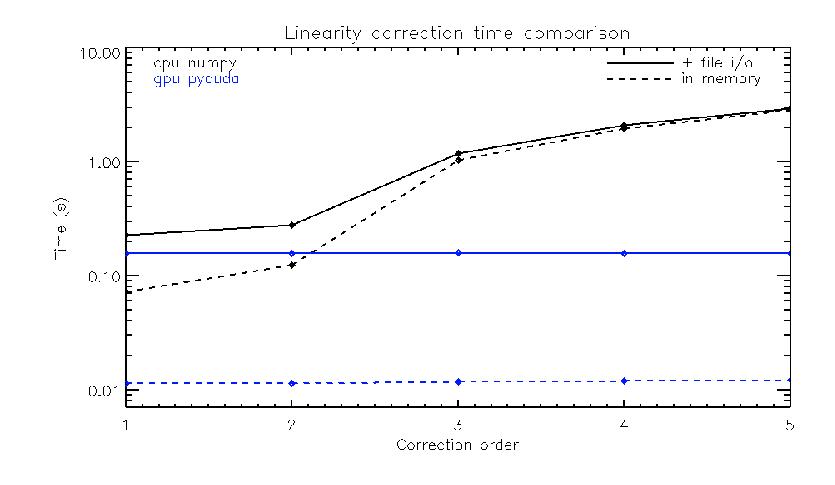
\includegraphics{part4/Warner_O31/O31_f1.eps}
\caption{File I/O is negligible compared to computation time on CPU for 3$^{rd}$ order and higher linearity corrections but dominates \ssindex{computing!GPU}GPU computation time!}
\end{figure}

We present a new, flexible data \ssindex{data!pipelines!reduction}pipeline model that combines \ssindex{computing!GPU}GPU-optimized algorithms with a new design that not only minimizes file I/O and byte-swapping operations, but also copying of data to and from the \ssindex{computing!GPU}GPU. 

\section{Methods \& Algorithms}

Our data \ssindex{data!pipelines!reduction}pipeline model is built in a \ssindex{computer languages!Python}python framework.  We choose \ssindex{computer languages!Python}python because it is an open-source, object-oriented language that has gained significant momentum within the astronomical community in recent years. There are a myriad of math and astronomy libraries that are freely available for \ssindex{computer languages!Python}python and supported by a large and active development community.  In addition, there are \ssindex{computer languages!Python}python modules that support \ssindex{data formats!XML}XML parsing and connecting to relational database management systems (RDBMS) such as \ssindex{databases!MySQL}mysql and \ssindex{databases!Postgres}PostgreSQL.  The \ssindex{libraries!PyCUDA}PyCUDA (\url{http://mathema.tician.de/software/pycuda}) module and \ssindex{computer languages!Python}python's native C-API allow us to easily integrate \ssindex{computing!GPU}GPU-optimized \ssindex{computing!architecture!CUDA}CUDA code into our data \ssindex{data!pipelines!reduction}pipeline, and finally, using \ssindex{computer languages!Python}python allows us to \ssindex{software!reuse}re-use some algorithms and classes, with only minor modifications, from previous data \ssindex{data!pipelines!reduction}pipelines, specifically the Florida Analysis Tool Born Of Yearning for high quality scientific data (FATBOY).  We use a machine with an \ssindex{NVIDIA}Nvidia 580 GTX GPU for all of our tests.

Our first challenge is to determine the best way to flexibly select and describe the data to be processed and the processes and options to be applied to the data.  Extensible Markup Language (\ssindex{data formats!XML}XML) is ideally suited for this task.  Using a simple \ssindex{data formats!XML}XML configuration file, the user will be able to describe their data, where it comes from, and what processes should be applied to the data.  The data can be retrieved either from an instrument's \ssindex{software!data handling}data handling system (DHS), from a local filesystem, or from an RDBMS.
 
In order to process data in near real-time at the telescope and provide rapid feedback via a quick-look mechanism, we select a data \ssindex{data!pipelines!reduction}pipeline design that operates on a per-image basis instead of a per-process basis.  At the telescope, we will have one image coming in from the instrument's DHS, and will want to apply previously created master calibration frames to this image immediately and send the resulting science data to the quick-look tool. Through this design and the use of recursive logic (Fig. 2), we can minimize file I/O to one read and one write per image.  All processes will be applied to the data in memory, with as many as possible combined into single steps on the \ssindex{computing!GPU}GPU to minimize both file I/O and memory copying (e.g., linearity correction, dark subtraction, flat division, and applying a bad pixel mask are all done in one method on the \ssindex{computing!GPU}GPU and then the resulting data is then copied back to host memory).  Master calibration frames are created once and then stored in memory and reused.

\begin{figure}[!ht]
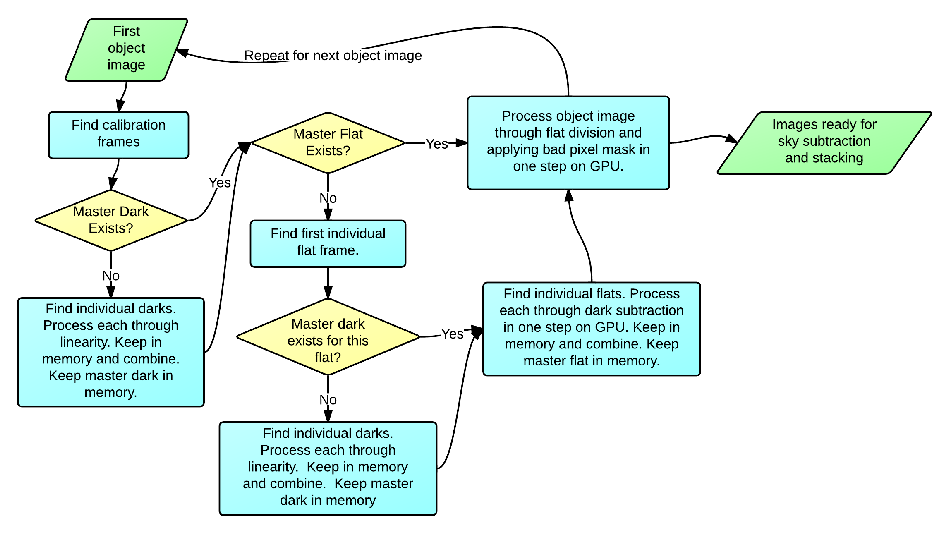
\includegraphics{part4/Warner_O31/O31_f2.eps}

\caption{Flow chart of recursive logic.  Master calibration frames are created once when they are first requested and then stored in memory and reused. All processes are applied to each frame in memory, with as many as possible performed at once on the \ssindex{computing!GPU}GPU, minimizing both file I/O and memory copying to and from the \ssindex{computing!GPU}GPU. }

\end{figure}


Finally, it is important that the data \ssindex{data!pipelines!reduction}pipeline design be customizeable and extensible so that new methods of both retrieving and processing data can be easily added to suit the needs of particular instruments.  Our design provides for this through the \ssindex{data formats!XML}XML configuration file combined with the ability to extend base classes and override methods as needed. 

\section{Results \& Conclusions}

Our preliminary results indicate that we can process a raw 2048 x 2048 near-infrared image all the way through sky subtraction and on-the-fly cosmic ray removal and save the result to disk in only 0.5 seconds!  This assumes that the master calibration frames (dark, flat field, bad pixel mask, and sky) for this image are already stored in memory.  The time required to create a master calibration frame depends upon the number of images that compose it, but should generally be on the order of 0.5 to 3 seconds.  With the exception of on-source skies, these calibration frames will only be created once per dataset and then kept in memory, minimizing overhead.

On-source skies are created from other object images at different positions in the dither pattern and increase in quality with more frames.  However, since the time required to create master sky frame is generally going to be shorter than the \ssindex{observing!exposure}exposure time for each observation, it will even be possible to recreate an iteratively better master sky and redo the sky subtraction after each observation in the dither pattern.  These iteratively better sky subtracted images can then be updated on disk and in the quick look tool, concurrent with continuing observations.  This will considerably optimize the observing process, resulting in huge savings of resources, money, and precious observing time.  We also believe that when applied to large archives of data, this design will make it possible to achieve a speed gain of as much as a factor of 30-40 over traditional CPU-based data \ssindex{data!pipelines!reduction}pipelines. 
